\section{Introducing differentiable binary arithmetic operations}
Our goal is to achieve arithmetic operations between the elements of a vector. Formally defined as \todo{Can this be more formally defined}.
\begin{equation}
x_1\circ_1 x_2 \circ_2 \cdots x_{k-1} \circ_{k-1} x_{k}\ |\ (x_1, \dots, x_k) \in \mathbf{x}, \mathbf{x} \in \mathbb{R}^n, \circ \in \{+, -, \cdot, \div \}
\label{eq:goal}
\end{equation}

The Neural Arithmetic Logic Unit (NALU)\cite{trask-nalu} attempts to solve equation \ref{eq:goal} by presenting two sub-units; the $\text{NAC}_{+}$ and $\text{NAC}_{\bullet}$ to exclusively represent either the $\{+, -\}$ or the $\{\cdot, \div \}$ operations.
The NALU attempts to have either $\text{NAC}_{+}$ or $\text{NAC}_{\bullet}$ selected exclusively, which could require the NALU to be applied multiple times (alternating between $\text{NAC}_{+}$ and $\text{NAC}_{\bullet}$) in order to represent the entire space of solutions for equation \ref{eq:goal}.

The $\text{NAC}_{+}$ and $\text{NAC}_{\bullet}$ are defined accordingly,

\begin{align}
W_{h_\ell, h_{\ell-1}} &= \tanh(\hat{W}_{h_\ell, h_{\ell-1}}) \sigma(\hat{M}_{h_\ell, h_{\ell-1}}) \label{eq:weight}\\
\textrm{NAC}_+:\ z_{h_\ell} &= \sum_{h_{\ell-1}=1}^{H_{\ell-1}} W_{h_{\ell}, h_{\ell-1}} z_{h_{\ell-1}} \label{eq:naca}\\
\textrm{NAC}_\bullet:\ z_{h_\ell} &= \exp\left(\sum_{h_{\ell-1}=1}^{H_{\ell-1}} W_{h_{\ell}, h_{\ell-1}} \label{eq:nacm}\log(|z_{h_{\ell-1}}| + \epsilon) \right)
\end{align}
where $\hat{\mathbf{W}}, \hat{\mathbf{M}} \in \mathbb{R}^{H_{\ell} \times H_{\ell-1}}$ are trainable weight matrices. These are then combined using tanh and sigmoid transformation to bias the parameters towards a $\{-1,0,1\}$ solution\todo{maybe visualize the function space}. Having $\{-1,0,1\}$ allows a linear layer to exactly emulate the binary $\{+, -\}$ operation between elements of a vector as used when computing the $\text{NAC}_{+}$.
The $\text{NAC}_{\bullet}$ extends the $\text{NAC}_{+}$ by using an exponential log transformation, which, with $\{-1,0,1\}$ weight values, becomes the $\{\cdot, \div \}$ operations (within $\epsilon$ precision).

The NALU combines these units with a gating mechanism $\mathbf{z} = \mathbf{g} \odot \text{NAC}_{+} + (1 - \mathbf{g}) \odot \text{NAC}_{\bullet}$ given $\mathbf{g} = \sigma(\mathbf{G} \mathbf{x})$. The idea is that the NALU should be a plug-and-play component in a neural network and has the ability to, with stochastic gradient descent and backpropagation, to learn the functionality in equation \ref{eq:goal}.

\subsection{Challenges of the NALU, $\text{NAC}_{+}$ and $\text{NAC}_{\bullet}$}
To simplify the problem we have chosen to leave out the gating mechanism and focus on the sub-units, assuming "oracle gating". \todo{We find this reasonable given ...}

We find that gating between $\text{NAC}_{+}$ and $\text{NAC}_{\bullet}$ is challenging to make converge and it it not obvious whether or not the gate could bias towards a specific sub-unit. We have not had any consistent success of convergence using the gating mechanism using the NALU or by combining our own proposed sub-units (NAU, NMU). We find that gating between $\text{NAC}_{+}$ and $\text{NAC}_{\bullet}$ is challenging. This is likely due to the vastly different gradients, causing addition to be learned much faster than multiplication.

In section \ref{sssec:weight} we analyse the gradients of equation \ref{eq:weight} and propose a cliped linear alternative, with a regularizer that biases towards $\{-1, 0, 1\}$. This results in an alternative addition unit called NAU.

In section \ref{sssec:nac-mul} we analyse the gradient of $\text{NAC}_{\bullet}$, and propose an alternative construction called NMU, that has a more well-behaved loss space.

In section \ref{sssec:nac-add-moments} we analyse the moments of $\text{NAC}_{+}$ and NAU, and derive the optimal weight initializations.

In section \ref{sssec:nac-mul-moments} we analyse the moments of $\text{NAC}_{\bullet}$ and NMU, and show that the NMU have a more well-behaved expectation and variance. \todo{Maybe remove this overview?}

\subsubsection{Weight matrix construction}\label{sssec:weight}

The weight matrix construction $\mathrm{tahn}(\hat{W}_{h_{\ell-1},h_\ell}) \sigma(\hat{M}_{h_{\ell-1},h_\ell})$ has the following properties that could make convergence challenging using gradient decent.

The loss gradient with respect to the weight matrices can be derived from equation \ref{eq:weight}.
\begin{equation}
\begin{aligned}
\frac{\partial \mathcal{L}}{\partial \hat{W}_{h_{\ell-1},h_\ell}} &= \frac{\partial \mathcal{L}}{\partial W_{h_{\ell-1},h_\ell}} (1 - \tanh^2(\hat{W}_{h_{\ell-1},h_\ell})) \sigma(\hat{M}_{h_{\ell-1},h_\ell}) \\
\frac{\partial \mathcal{L}}{\partial \hat{M}_{h_{\ell-1},h_\ell}} &= \frac{\partial \mathcal{L}}{\partial W_{h_{\ell-1},h_\ell}} \tanh(\hat{W}_{h_{\ell-1},h_\ell}) \sigma(\hat{M}_{h_{\ell-1},h_\ell}) (1 - \sigma(\hat{M}_{h_{\ell-1},h_\ell}))
\end{aligned}
\label{eq:nac-weight-gradient}
\end{equation}

The gradient $E\left[\nicefrac{\partial \mathcal{L}}{\partial \hat{M}_{h_{\ell-1},h_\ell}}\right] = 0$ can be problematic as we prefer zero having a zero mean expectation of our output.
Something that can only be ensured with $E[\hat{W}_{h_{\ell-1},h_\ell}] = 0$ \cite{glorot-initialization}.

In our empirical analysis we find that equation \ref{eq:weight} does not create the desired bias for $\{-1, 0, 1\}$, as it doesn't converge towards those values.

To create a bias and prevent the gradient challenges of equation \ref{eq:nac-weight-gradient} we propose a simple clamped linear construction with an out-of-bound regularizer $\mathcal{R}_{\ell,\mathrm{oob}}$ to force $\hat{W}$ to be within $[-1, 1]$ and ensure that the gradient is always present.
\begin{equation}
\begin{aligned}
W_{h_{\ell-1},h_\ell} &= \min(\max(\hat{W}_{h_{\ell-1},h_\ell}, -1), 1), \\
\mathcal{R}_{\ell,\mathrm{bias}} &= \frac{1}{H_\ell + H_{\ell-1}} \sum_{h_\ell=1}^{H_\ell} \sum_{h_{\ell-1}=1}^{H_{\ell-1}} \hat{W}_{h_{\ell-1},h_\ell}^2 (1 - |\hat{W}_{h_{\ell-1},h_\ell}|)^2 \\
\mathcal{R}_{\ell,\mathrm{oob}} &= \frac{1}{H_\ell + H_{\ell-1}} \sum_{h_\ell=1}^{H_\ell} \sum_{h_{\ell-1}=1}^{H_{\ell-1}} \max(|\hat{W}_{h_{\ell-1},h_\ell}| - 1, 0)^2 \\
\textrm{NAU}:\ z_{h_\ell} &= \sum_{h_{\ell-1}=1}^{H_{\ell-1}} W_{h_{\ell}, h_{\ell-1}} z_{h_{\ell-1}} \\
\mathcal{L} &= \hat{\mathcal{L}} + \lambda_{\mathrm{bias}} \mathcal{R}_{\ell,\mathrm{bias}} + \lambda_{\mathrm{oob}} \mathcal{R}_{\ell,\mathrm{oob}}
\end{aligned}
\end{equation}

\subsubsection{Challenges of division} \label{sssec:nac-mul}

The $\text{NAC}_{\bullet}$, as formulated in equation \ref{eq:nacm}, has the ability to learn exact multiplication and division of elements from a vector if the weights of $W_{h_{\ell-1},h_\ell}$ are one of $\{-1, 0, 1\}$.

However, backpropagation through the $\text{NAC}_{\bullet}$ unit reveals that if $|z_{h_{\ell-1}}|$ is near zero, $W_{h_{\ell-1},h_\ell}$ is negative and $\epsilon$ is small, the gradient term will explode and oscillate between large postive and large negative values, which can be problematic in optimization \cite{adam-optimization}, as visualized in figure \ref{fig:nac-mul-eps-issue}.

\begin{align}
%\frac{\partial \mathcal{L}}{\partial W_{h_{\ell}, h_{\ell - 1}}} &= \frac{\partial \mathcal{L}}{\partial z_{h_\ell}} \frac{\partial z_{h_\ell}}{\partial W_{h_{\ell}, h_{\ell - 1}}} = \frac{\partial \mathcal{L}}{\partial z_{h_\ell}} z_{h_\ell} \log(|z_{h_{\ell-1}}| + \epsilon) \label{eq:dw}\\
\frac{\partial \mathcal{L}}{\partial z_{h_{\ell-1}}} &= \sum_{h_\ell = 1}^{H_\ell} \frac{\partial \mathcal{L}}{\partial z_{h_\ell}} \frac{\partial z_{h_\ell}}{\partial z_{h_{\ell-1}}} = \sum_{h_\ell = 1}^{H_\ell} \frac{\partial \mathcal{L}}{\partial z_{h_\ell}} z_{h_\ell} W_{h_\ell, h_{\ell-1}} \frac{\mathrm{sign}(z_{h_{\ell-1}})}{|z_{h_{\ell-1}}| + \epsilon}\label{eq:dz}
\end{align}
(see full derivation in Appendix \ref{sec:appendix:gradient-derivatives:gradient-nac-mul})

This is not an issue for for positive values of $W_{h_{\ell-1},h_\ell}$ (multiplication), as $z_{h_{\ell}}$ and $z_{h_{\ell-1}}$ will be correlated causing the terms $z_{h_\ell}$ and $\frac{\mathrm{sign}(z_{h_{\ell-1}})}{|z_{h_{\ell-1}}| + \epsilon}$ to cancel out.
%However, for negative values of $W_{h_{\ell-1},h_\ell}$ the terms will be negatively correlated causing an unwanted loss space, which is visualized in figure \ref{fig:nac-mul-eps-issue}.

\begin{figure}[H]
\centering
\begin{subfigure}{.33\textwidth}
  \centering
  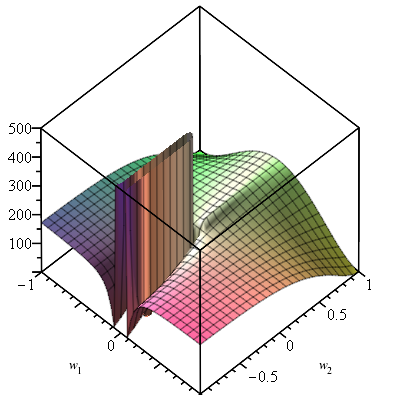
\includegraphics[width=\linewidth]{graphics/nac-mul-eps-1em7.png}
  \caption{$\epsilon = 10^{-7}$}
\end{subfigure}%
\begin{subfigure}{.33\textwidth}
  \centering
  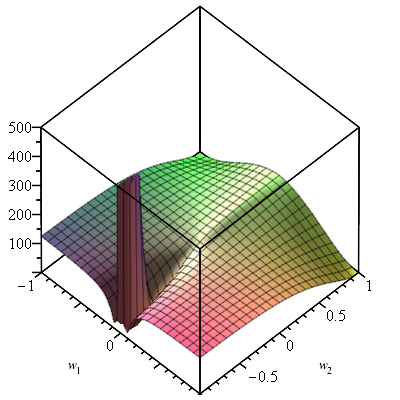
\includegraphics[width=\linewidth]{graphics/nac-mul-eps-1em1.png}
  \caption{$\epsilon = 0.1$}
\end{subfigure}
\begin{subfigure}{.33\textwidth}
  \centering
  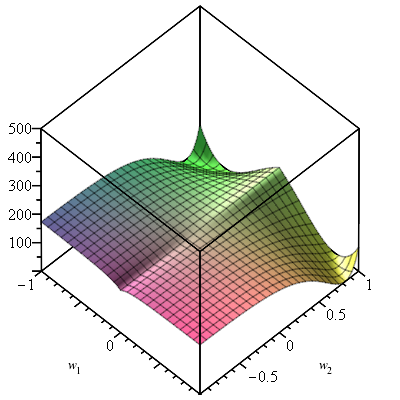
\includegraphics[width=\linewidth]{graphics/nac-mul-eps-1.png}
  \caption{$\epsilon = 1$}
\end{subfigure}
\caption{RMS loss curvature for a $\mathrm{NAC}_{+}$ layer followed by a $\mathrm{NAC}_{\bullet}$ layer. The weight matrices constrained are to $\mathbf{W}_1 = \left[\protect\begin{smallmatrix}
w_1 & w_1 & 0 & 0 \\
w_1 & w_1 & w_1 & w_1
\protect\end{smallmatrix}\right]$, $\mathbf{W}_2 = \left[\protect\begin{smallmatrix}
w_2 & w_2
\protect\end{smallmatrix}\right]$. The problem is $x = \left(1, 1.2, 1.8, 2\right), t = 13.2$. Desired solution is $w_1 = w_2 = 1$, although this problem have additional undesired solutions.}
\label{fig:nac-mul-eps-issue}
\end{figure}

These observations are particular problematic when considering that $E[z_{h_{\ell-1}}] = 0$ is a desired property when initializing \cite{glorot-initialization}. An alternative multiplication operator must thus be able to not explode for $z_{h_{\ell-1}}$ near zero. To that end we propose a new neural multplication units (NMU): 

\begin{equation}
\begin{aligned}
&W_{h_{\ell-1},h_\ell} = \min(\max(\hat{W}_{h_{\ell-1},h_\ell}, 0), 1), \\
&\mathcal{R}_{\ell,\mathrm{bias}} = \frac{1}{H_\ell + H_{\ell-1}} \sum_{h_\ell=1}^{H_\ell} \sum_{h_{\ell-1}=1}^{H_{\ell-1}} \hat{W}_{h_{\ell-1},h_\ell}^2 (1 - \hat{W}_{h_{\ell-1},h_\ell})^2 \\
&\mathcal{R}_{\ell,\mathrm{oob}} = \frac{1}{H_\ell + H_{\ell-1}} \sum_{h_\ell=1}^{H_\ell} \sum_{h_{\ell-1}=1}^{H_{\ell-1}} \max\left(\left|\hat{W}_{h_{\ell-1},h_\ell} - \frac{1}{2}\right| - \frac{1}{2}, 0\right)^2 \\
\textrm{NMU}:\ &z_{h_\ell} = \prod_{h_{\ell-1}=1}^{H_{\ell-1}} \left(W_{h_{\ell-1},h_\ell} z_{h_{\ell-1}} + 1 - W_{h_{\ell-1},h_\ell} \right)
\end{aligned}
\end{equation}

This units does not support division, but supporting division is likely infeasible if $z_{h_{\ell-1}}$ near zero should not cause explosions. The NALU paper also shows that division doesn't work well for their unit, hence very little is lost here \cite{trask-nalu}. On the other hand, this unit construction understand the difference between a negative and a positive $z_{h_{\ell-1}}$ values, which should be considered an added bonus, as this allows extrapolations into the negative input range.

The gradients weight gradient and backpropagation term of the NMU are (see details in Appendix \ref{sec:appendix:gradient-derivatives:gradient-nmu}):
\begin{equation}
\begin{aligned}
\frac{\partial \mathcal{L}}{\partial W_{h_{\ell}, h_{\ell - 1}}} &= \frac{\partial \mathcal{L}}{\partial z_{h_\ell}} \frac{\partial z_{h_\ell}}{\partial W_{h_{\ell}, h_{\ell - 1}}} = \frac{\partial \mathcal{L}}{\partial z_{h_\ell}} \frac{z_{h_\ell}}{W_{h_{\ell-1},h_\ell} z_{h_{\ell-1}} + 1 - W_{h_{\ell-1},h_\ell}} \left(z_{h_{\ell-1}} - 1\right) \\
\frac{\partial \mathcal{L}}{\partial z_{h_{\ell-1}}} &= \sum_{h_\ell = 1}^{H_\ell} \frac{\partial \mathcal{L}}{\partial z_{h_\ell}} \frac{\partial z_{h_\ell}}{\partial z_{h_{\ell-1}}} = \sum_{h_\ell = 1}^{H_\ell} \frac{z_{h_\ell}}{W_{h_{\ell-1},h_\ell} z_{h_{\ell-1}} + 1 - W_{h_{\ell-1},h_\ell}} W_{h_{\ell-1},h_\ell}
\end{aligned}
\end{equation}

These is much more well-behaved. Note also that the fraction does not explode for $z_{h_{\ell-1}}$ close to zero, as the denominator simply cancels out a term in $z_{h_\ell}$.

\begin{figure}[H]
\centering
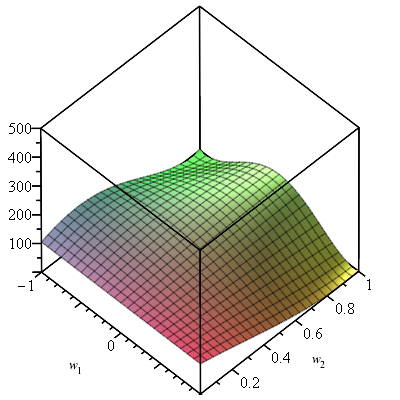
\includegraphics[width=0.33\linewidth]{graphics/nac-mul-nmu.png}
\caption{RMS loss curvature (without regularization) for a $\mathrm{NAC}_{+}$ layer followed by an $\mathrm{NMU}$ layer. Otherwise, the setup is identical to that in Figure \ref{fig:nac-mul-eps-issue}.}
\end{figure}

\subsubsection{Moments and initialization}

Initialization is important to consider for fast and consistent convergence \cite{glorot-initialization}.

Our proposed NAU, can be initialize using Glorot initialzation as it is just a linear layer. The $\mathrm{NAC}_{+}$ unit can also achieve an ideal initialization, although it is less trivial (details in Appendix \ref{sec:appendix:moments:weight-matrix-construction}).

Using second order multivariate Taylor approximation and some assumptions of uncorrelated stochastic variables, the expectation of $\mathrm{NAC}_{\bullet}$ can be estimated to be
\begin{equation}
E[z_{h_\ell}] \approx \left(1 + \frac{1}{2} Var[W_{h_\ell, h_{\ell-1}}] \log(|E[z_{h_{\ell-1}}]| + \epsilon)^2\right)^{H_{\ell-1}} \Rightarrow E[z_{h_\ell}] > 1 \label{eq:nac-mul:expectation}
\end{equation}
(proof in Appendix \ref{sec:appendix:moments:nac-mul}). An ideal initialization should satisfy $E[z_{h_\ell}] = 0$ \cite{glorot-initialization}, which the expectation for $\mathrm{NAC}_{\bullet}$ can't.

Our proposed NMU when initialized with $E[W_{h_{\ell}, h_{\ell - 1}}] = \nicefrac{1}{2}$ has an expectation of
\begin{equation}
E[z_{h_\ell}] \approx \left(\frac{1}{2}\right)^{H_{\ell-1}}
\end{equation}
which is not zero, but does approach zero for $H_{\ell-1} \rightarrow \infty$ (proof in Appendix \ref{sec:appendix:moments:nmu}).

The variance is also more well-behaved, but does similarly to $\mathrm{NAC}_{\bullet}$ not provide a input-independent initialization strategy (proof in Appendix \ref{sec:appendix:moments:nac-mul} and \ref{sec:appendix:moments:nmu}). We propose initializing with $Var[W_{h_{\ell-1},h_\ell}] = \frac{1}{4}$, as this provides an ideal initialization if $Var[z_{h_{\ell-1}}] = 1$ and $H_{\ell-1}$ is large (see proof in Appendix \ref{sec:appendix:moments:nmu:initialization}).

\subsubsection{Moments and initialization for addition} \label{sssec:nac-add-moments}
\todo{Maybe put this entire section in appendix?}

Initialization is important for fast and consistent convergence. The desired properties are according to Glorot et al. \cite{glorot-initialization}:
\begin{equation}
\begin{aligned}
E[z_{h_\ell}] &= 0 & E\left[\frac{\partial \mathcal{L}}{\partial z_{h_{\ell-1}}}\right] &= 0 \\
Var[z_{h_\ell}] &= Var\left[z_{h_{\ell-1}}\right] &
Var\left[\frac{\partial \mathcal{L}}{\partial z_{h_{\ell-1}}}\right] &= Var\left[\frac{\partial \mathcal{L}}{\partial z_{h_{\ell}}}\right]
\end{aligned}
\end{equation}

The $\mathrm{NAU}$ layer is trivial, as this is just a linear layer. Thus the result from Glorot et al. ($Var[W_{h_{\ell-1},h_{\ell}}] = \frac{2}{H_{\ell-1} + H_{\ell}}$) can be used \cite{glorot-initialization}.

However, the original $\mathrm{NAC}_{+}$ unit is less trivial as $W_{h_{\ell-1},h_{\ell}}$ is not sampled directly. Assuming that $\hat{W}_{h_\ell, h_{\ell-1}} \sim \mathrm{Uniform}[-r, r]$ and $\hat{M}_{h_\ell, h_{\ell-1}} \sim \mathrm{Uniform}[-r, r]$ then the variance can be derived (see proof in Appendix \ref{sec:appendix:moments:weight-matrix-construction}) to be:
\begin{equation}
Var[W_{h_{\ell-1},h_{\ell}}] = \frac{1}{2r} \left(1 - \frac{\tanh(r)}{r}\right) \left(r - \tanh\left(\frac{r}{2}\right)\right)
\end{equation}
One can the solve for $r$, given the desired variance.

\subsubsection{Moments and initialization for multiplication} \label{sssec:nac-mul-moments}
\todo{Maybe put this entire section in appendix?}

Using second order multivariate Taylor approximation and some assumptions\todo{put in assumptions in appendix} of uncorrelated stochastic variables, the expectation and variance of the $\mathrm{NAC}_{\bullet}$ layer can be estimated to:
\begin{equation}
\begin{aligned}
f(c_1, c_2) &= \left(1 + c_1 \frac{1}{2} Var[W_{h_\ell, h_{\ell-1}}] \log(|E[z_{h_{\ell-1}}]| + \epsilon)^2\right)^{c_2\ H_{\ell-1}} \\
E[z_{h_\ell}] &\approx f\left(1, 1\right) \\
Var[z_{h_2}] &\approx f\left(4, 1\right) - f\left(1, 2\right) \\
E\left[\frac{\partial \mathcal{L}}{\partial z_{h_{\ell-1}}}\right] &= 0 \\
Var\left[\frac{\partial \mathcal{L}}{\partial z_{h_{\ell-1}}}\right] &\approx Var\left[\frac{\partial \mathcal{L}}{\partial z_{h_{\ell}}}\right] H_{\ell}\ f\left(4, 1\right)\ Var[W_{h_{\ell}, h_{\ell-1}}] \\
&\cdot \left(\frac{1}{\left(|E[z_{h_{\ell-1}}]| + \epsilon\right)^2} + \frac{3}{\left(|E[z_{h_{\ell-1}}]| + \epsilon\right)^4} Var[z_{h_{\ell-1}}]\right)
\end{aligned}
\end{equation}

This is problematic because $E[z_{h_\ell}] \ge 1$, and the variance explodes for $E[z_{h_{\ell-1}}] = 0$ which is normally a desired property.

For our proposed NMU, the expectation and variance can be derived (see proof in Appendix \ref{sec:appendix:moments:nmu}) using the same assumptions as before, although no Taylor approximation is required:
\begin{equation}
\begin{aligned}
E[z_{h_\ell}] &\approx \left(\frac{1}{2}\right)^{H_{\ell-1}} \\
E\left[\frac{\partial \mathcal{L}}{\partial z_{h_{\ell-1}}}\right] &\approx 0 \\
Var[z_{h_\ell}] &\approx \left(Var[W_{h_{\ell-1},h_\ell}] + \frac{1}{4}\right)^{H_{\ell-1}} \left(Var[z_{h_{\ell-1}}] + 1\right)^{H_{\ell-1}} - \left(\frac{1}{4}\right)^{H_{\ell-1}} \\
Var\left[\frac{\partial \mathcal{L}}{\partial z_{h_{\ell-1}}}\right] &\approx Var\left[\frac{\partial \mathcal{L}}{\partial z_{h_\ell}}\right] H_\ell \\
& \cdot \left( \left(Var[W_{h_{\ell-1},h_\ell}] + \frac{1}{4}\right)^{H_{\ell-1}} \left(Var[z_{h_{\ell-1}}] + 1\right)^{H_{\ell-1}-1} - \left(\frac{1}{4}\right)^{H_{\ell-1}}\right)
\end{aligned}
\end{equation}\todo{consider throwing in appendix}

These expectations are much more well behaved. It is properly unlikely to expect that the expectation can become zero, since the identity for multiplication is 1. However, for a large $H_{\ell-1}$ it will be near zero.

The variance is also more well-behaved, but does not provide a input-independent initialization strategy. We propose initializing with $Var[W_{h_{\ell-1},h_\ell}] = \frac{1}{4}$, as this is the solution to $Var[z_{h_\ell}] = Var[z_{h_{\ell-1}}]$ assuming $Var[z_{h_{\ell-1}}] = 1$ and a large $H_{\ell-1}$ (see proof in Appendix \ref{sec:appendix:moments:nmu:initialization}). However, feel free to compute more exact solutions.

